%
% federpendel.tex
%
% (c) 2025 Prof Dr Andreas Müller
%
\documentclass[tikz]{standalone}
\usepackage{amsmath}
\usepackage{times}
\usepackage{txfonts}
\usepackage{pgfplots}
\usepackage{csvsimple}
\usetikzlibrary{arrows,intersections,math}
\usetikzlibrary{decorations.pathmorphing,patterns}
\begin{document}


%erste Version
%\begin{tikzpicture}[>=latex,thick]
    % Koordinatensystem
 %   \draw[->] (-2,0) -- (2,0) node[right] {$x$};
  %  \draw[->] (0,-2) -- (0,2) node[above] {$y$};
    
    % Feder
   % \draw[thick] (0,1.5) -- (0,1.2);
    %\draw[thick, decorate, decoration={coil, aspect=0.5, %segment length=4mm, amplitude=2mm}] (0,1.2) -- (0,-0.5);
    
    % Körper
    %\filldraw[blue] (0,-0.5) circle (0.3) node[below] {$m$};
    
    % Kräfte
    %\draw[->, thick, red] (0,-0.5) -- (0,-1.5) node[right] {$\vec{F}_G$};
    %\draw[->, thick, green] (0,-0.5) -- (0,0.5) node[right] %{$\vec{F}_S$};
    
    % Aufhängung
    %\draw[thick] (-0.5,1.5) -- (0.5,1.5);
%\end{tikzpicture}


	
		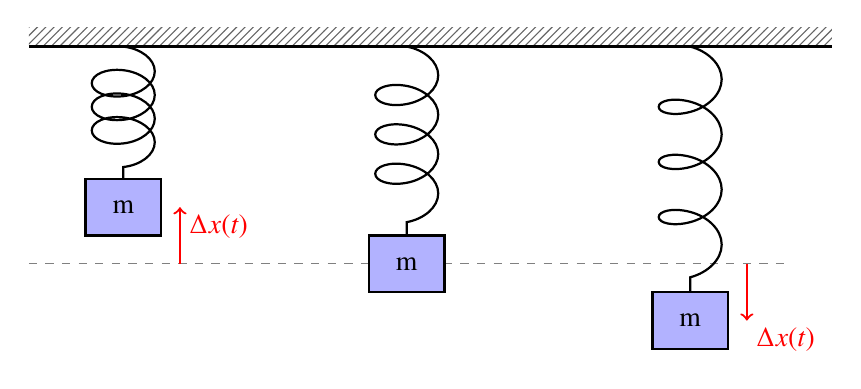
\begin{tikzpicture}[scale=1.2]
			
			% Decke
			\fill[pattern=north east lines, pattern color=black!60] (-4,0) rectangle (4.5,0.2);
			\draw[thick] (-4,0) -- (4.5,0);
			
			% Referenzlinie auf Höhe der mittleren Masse
			\draw[dashed, gray] (-4,-2.3) -- (4,-2.3);
			
			% === Linkes Pendel (gestaucht) ===
			\begin{scope}[shift={(-3,0)}]
				% Feder mit 4 Windungen in 1.6cm
				\draw[decorate, decoration={
					coil,
					aspect=0.6,
					segment length=3mm,   % 16mm/4
					amplitude=4mm},
				thick] (0,0) -- (0,-1.4);
				% Masse
				\draw[fill=blue!30, thick] (-0.4,-1.4) rectangle (0.4,-2);
				\node at (0,-1.7) {m};
				% Pfeil nach oben (von mittlerer Massehöhe)
				\draw[->, thick, red] (0.6,-2.3) -- (0.6,-1.7);
				\node[right, red] at (0.6,-1.9) {$\Delta x(t)$};
			\end{scope}
			
			% === Mittleres Pendel (Ruhelage) ===
			\begin{scope}
				% Feder mit 4 Windungen in 2.0cm
				\draw[decorate, decoration={
					coil,
					aspect=0.6,
					segment length=5mm,   % 20mm/4
					amplitude=4mm},
				thick] (0,0) -- (0,-2.0);
				\draw[fill=blue!30, thick] (-0.4,-2.0) rectangle (0.4,-2.6);
				\node at (0,-2.3) {m};
			\end{scope}
			
			% === Rechtes Pendel (gestreckt) ===
			\begin{scope}[shift={(3,0)}]
				% Feder mit 4 Windungen in 2.8cm
				\draw[decorate, decoration={
					coil,
					aspect=0.6,
					segment length=7mm,   % 28mm/4
					amplitude=4mm},
				thick] (0,0) -- (0,-2.6);
				\draw[fill=blue!30, thick] (-0.4,-2.6) rectangle (0.4,-3.2);
				\node at (0,-2.9) {m};
				% Pfeil nach unten (von mittlerer Massehöhe)
				\draw[->, thick, red] (0.6,-2.3) -- (0.6,-2.9);
				\node[right, red] at (0.6,-3.1) {$\Delta x(t)$};
			\end{scope}
			
		\end{tikzpicture}
	




\end{document}
